\documentclass[tikz,border=9pt]{standalone}
\usepackage[utf8]{inputenc}
\usepackage[OT4,plmath]{polski}
\usepackage{amsmath}
\begin{document}
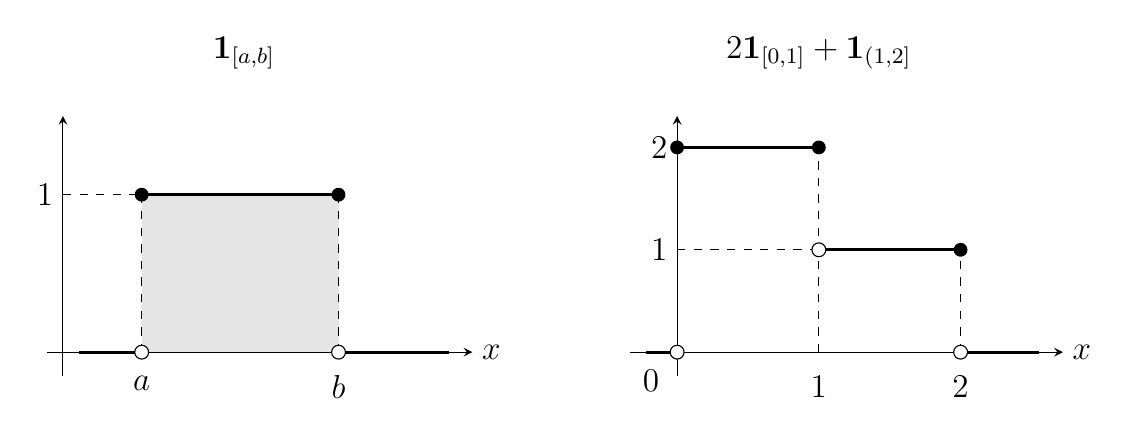
\begin{tikzpicture}[font=\large,>=stealth]
  \begin{scope}
    \node at (2.3,3.8) {$\mathbf{1}_{[a,b]}$};
    \fill[black!10] (1,0) rectangle (3.5,2.0);
    \draw[->] (-0.2,0)--(5.2,0) node[right] {$x$};
    \draw[->] (0,-0.3)--(0,3.0);
    \draw[very thick] (0.2,0)--(1,0);
    \draw[very thick] (1,2)--(3.5,2);
    \draw[very thick] (3.5,0)--(4.9,0);
    \draw[dashed] (1,0)--(1,2) (3.5,0)--(3.5,2) (0,2)--(1,2);
    \foreach \x in {1,3.5} {
      \node[circle,draw,fill=white,inner sep=0pt,minimum size=5pt] at (\x,0) {};
      \node[circle,fill,inner sep=0pt,minimum size=5pt] at (\x,2) {};
    }
    \node[left] at (0,2) {$1$};
    \node[below=5pt] at (1,0) {$a$};
    \node[below=5pt] at (3.5,0) {$b$};
  \end{scope}
  \begin{scope}[xshift=7.8cm]
    \node at (1.8,3.8) {$2\mathbf{1}_{[0,1]}+\mathbf{1}_{(1,2]}$};
    \draw[->] (-0.6,0)--(4.9,0) node[right] {$x$};
    \draw[->] (0,-0.3)--(0,3.0);
    \draw[very thick] (-0.4,0)--(0,0);
    \draw[very thick] (0,2.6)--(1.8,2.6);
    \draw[very thick] (1.8,1.3)--(3.6,1.3);
    \draw[very thick] (3.6,0)--(4.6,0);
    \draw[dashed] (1.8,0)--(1.8,2.6) (3.6,0)--(3.6,1.3);
    \draw[dashed] (0,1.3)--(1.8,1.3);
    \foreach \x/\y in {0/0,1.8/1.3,3.6/0}
      \node[circle,draw,fill=white,inner sep=0pt,minimum size=5pt] at (\x,\y) {};
    \foreach \x/\y in {0/2.6,1.8/2.6,3.6/1.3}
      \node[circle,fill,inner sep=0pt,minimum size=5pt] at (\x,\y) {};
    \node[left] at (0,1.3) {$1$};
    \node[left] at (0,2.6) {$2$};
    \node[below left=3pt] at (0,0) {$0$};
    \node[below=5pt] at (1.8,0) {$1$};
    \node[below=5pt] at (3.6,0) {$2$};
  \end{scope}
\end{tikzpicture}
\end{document}
